\begin{figure}[ht!]
\centering
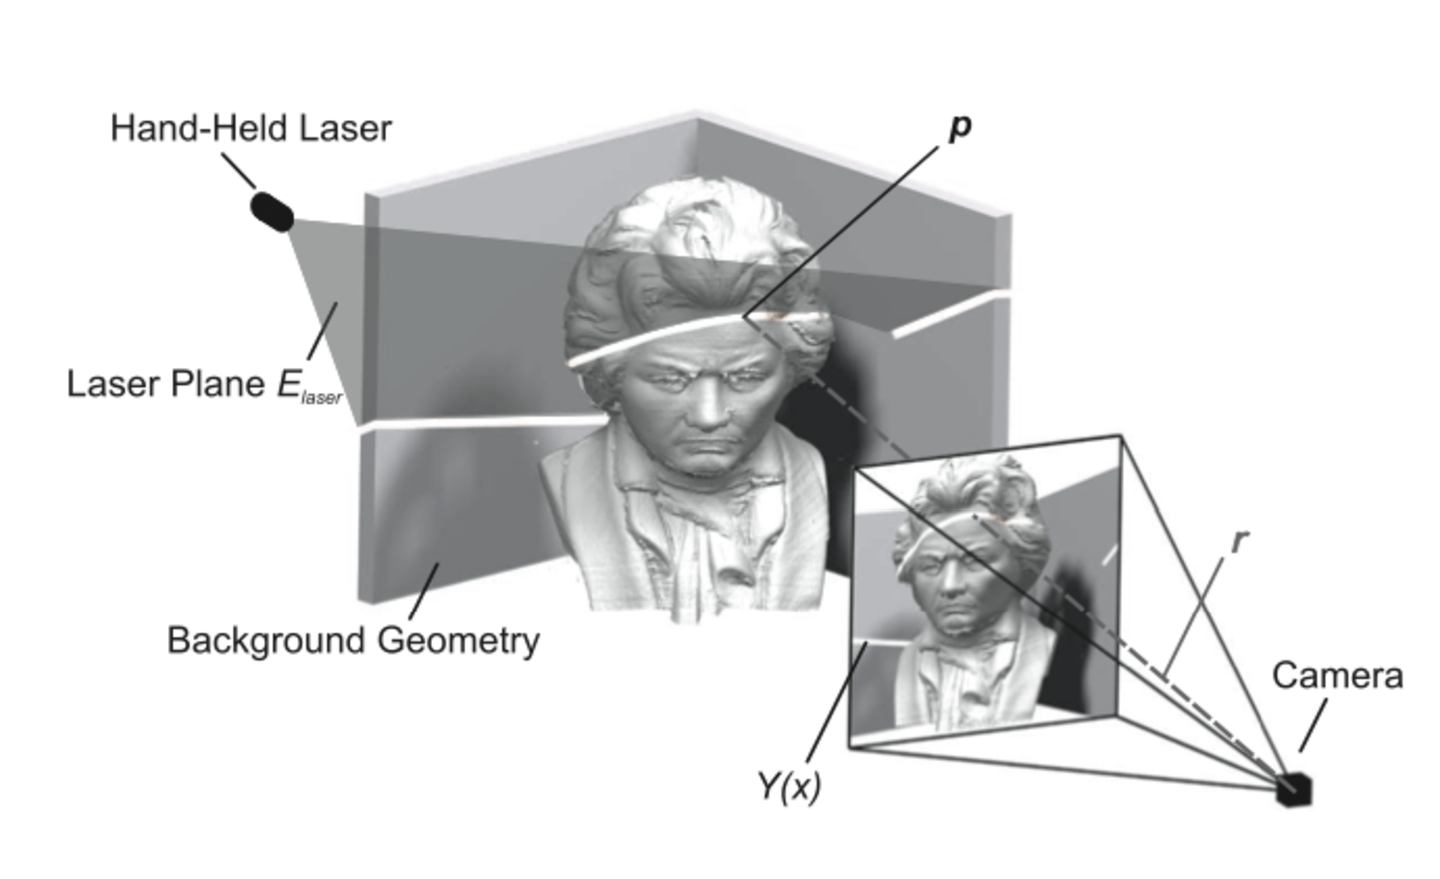
\includegraphics[width=0.9\linewidth]{figures/pointcloudpaper}
\caption{Laser Triangulation \cite{winkelbach:2006}}
\label{figure:triangulation}
\end{figure}

The first step is to use the calculated camera extrinsics ($R \mid T$) for each side of the target object along with the intrinsic parameters ($A$) to transform each laser pixel ($P_c$) into 3D laser surface points ($P_w$) using equation \ref{equation:3dlaserpoint}. The laser pixel points are expressed in the homogenous coordinate system. 

\begin{align}
	\label{equation:3dlaserpoint}				
	P_w &= 	\underbrace{s \times R^{-1} 
 					 							\times A^{-1}
 												\times P_c
										 }_\text{$\overrightarrow{b}$}
					- 
					\underbrace{
											R^{-1} \times T					
										 }_\text{$\overrightarrow{a}$} \\
	\text{where}~
	P_c &= \begin{pmatrix}
						u \\ 
						v \\
						1 \\
				 \end{pmatrix}, 
	\overrightarrow{a} = \begin{pmatrix}
													a_x \\
													a_y \\
													a_z \\
												\end{pmatrix}, 
	\overrightarrow{b} = \begin{pmatrix}
													b_x \\
													b_y \\
													b_z \\
												\end{pmatrix} \notag \\ 
  \text{and}~ s &= \frac{a_z}{b_z} \notag
\end{align}

Next in order to bring all the laser surface points into a common coordinate system, we transformed all the 3D laser points from the right side of the target object to the coordinate system of the left side using equation \ref{equation:right2left}

\begin{align}
	\label{equation:right2left}				
	P_{l} &= R_1^{-1} \times P_{r} - R_1^{-1}T_1 \\
	\text{where}~ 
	P_{r} &= \begin{bmatrix}
									R_2 \mid T_2
 				  \end{bmatrix} \times P_w \notag
\end{align}

With all the 3D laser surface points in a common coordinate system, we randomly choose 3 points to generate the laser plane equation. Using the coefficients of this equation, we could define the normal to the plane $(\overrightarrow{N})$ using equation \ref{equation:laserplaneequation}.

\begin{align}
	\label{equation:laserplaneequation}				
	A_x + B_y + C_z + D &= 0 \\
	\text{where}~
	 \overrightarrow{N} &=
	 \begin{pmatrix}
	  A \\
	  B \\
	  C \\
	 \end{pmatrix} \notag
\end{align}

The last step is to use the target object pixels $(P_c)$ and intersect them with the laser plane equation represented by the normal $(\overrightarrow{N})$ to obtain the 3D surface points of the target object $(P_w)$ as shown in figure \ref{figure:triangulation} using equation \ref{equation:3dobjectpoint}

\begin{align}
	\label{equation:3dobjectpoint}				
	P_w &= s \times R^{-1} 
 					 \times A^{-1} 
					 \times P_c
					- R^{-1} \times T \\
	\text{where}~	
	s &= \frac{\overrightarrow{N}\times\overrightarrow{a} - D}
						{\overrightarrow{b}\times\overrightarrow{N}}
  ~\text{and}~ P_c = \begin{pmatrix}
												u \\
												v \\
												1 \\
										 \end{pmatrix} \notag
\end{align}				

In addition, we used OpenCV routine \texttt{cvGet2D()} to retrieve the RGB color information for each object pixel and mapped it to the calculated corresponding 3D object surface point. We used the reference image as the source for retrieving the original color information since that image does not have a laser line sweeping the target object.